\documentclass{article}
\usepackage[utf8]{inputenc}

\title{MATH3160 — Portfolio 5.5, 5.6}
\author{Mike Medved}
\date{November 9th, 2022}

\usepackage{color}
\usepackage{amsthm}
\usepackage{amssymb} 
\usepackage{amsmath}
\usepackage[margin=1in]{geometry} 
\usepackage{listings}
\usepackage[dvipsnames]{xcolor}
\usepackage{tikz}

\newtheorem*{thm}{Theorem}

\begin{document}

\maketitle

\section{Deliverables}

\subsection{Geometric Random Variable}

A geometric random variable represents the number of Bernoulli trials, $Bern(p)$, until the first successful trial occurs.

$\hfill \break$
\textbf{Definition:} Let $X$ be a geometric random variable with parameter $p \in (0, 1)$ written as $X \sim Geom(p)$.

\begin{table}[!htb]
    \centering
    \begin{tabular}{|l|l|l|l|l|}
        \hline
        \multicolumn{1}{|c|}{\textit{Im X}} & \multicolumn{1}{c|}{\textit{pmf}} & \multicolumn{1}{c|}{\textit{E[X]}} & \multicolumn{1}{c|}{\textit{Var(X)}} & \multicolumn{1}{c|}{\textit{mgf}} \\ \hline
        $\mathbb{N}$                          & $p*q^{k-1}$                         & $\dfrac{1}{p}$                        & $\dfrac{q}{p^2}$                        & $\dfrac{pe^t}{1-qe^t}$               \\ \hline
    \end{tabular}
    \caption{Properties of $X \sim Geom(p)$}
\end{table}

$\hfill \break$
The mgf of a geometric random variable takes values $t$ such that $t \in \left(-\infty, ln\left(\frac{1}{q}\right)\right)$.

\subsubsection{Geometric Random Variable Mass Plot}

\begin{figure}[!htb]
    \begin{center}
        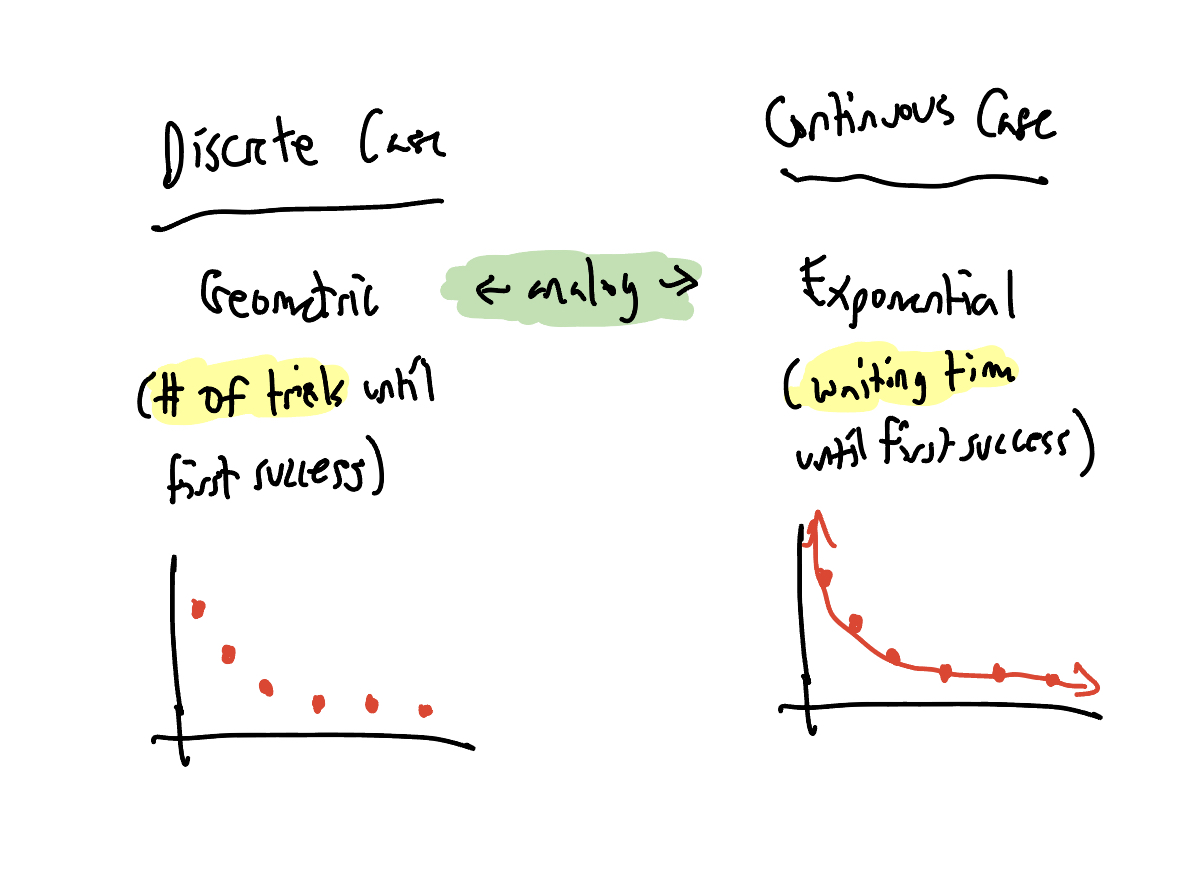
\includegraphics[height=2in]{q1.jpeg}
        \caption{Discrete vs Continuous Plot for $X \sim Geom(p)$, $X \sim Exp(p)$}
    \end{center}
\end{figure}

\newpage
\subsection{Memoryless Property}

The memoryless property states that the probability of a geometric random variable is independent of the number of trials that have already occurred.

$$
P(X > n + m | x > m) = P(X > n)
$$

\begin{center}
    for all $m, n \in \mathbb{N}; m, n > 1$.
\end{center}

$\hfill \break$
The geometric random variable is the only discrete random variable for which the memoryless property holds true. Additionally, we have found that $P(X > n) = q^n$

\subsection{Poisson Random Variable}

A poisson random variable represents the number of events that occur in a fixed interval of time.

$\hfill \break$
\textbf{Definition:} Let $X$ be a poisson random variable with parameter $\lambda \in \mathbb{R}^+$ written as $X \sim \rho(\lambda)$.

\begin{table}[!htb]
    \centering
    \begin{tabular}{|l|l|l|l|l|l|}
        \hline
        \multicolumn{1}{|c|}{\textit{Im X}} & \multicolumn{1}{|c|}{Taylor($e^x$)} & \multicolumn{1}{c|}{\textit{pmf}} & \multicolumn{1}{c|}{\textit{E[X]}} & \multicolumn{1}{c|}{\textit{Var(X)}} & \multicolumn{1}{c|}{\textit{mgf}} \\ \hline
        $\mathbb{N}$                         & $\displaystyle\sum_{n=0}^{\mathbb{R}} \frac{x^n}{n!}$ & $\frac{\lambda^k}{k!}\cdot e^{-\lambda}$                         & $\lambda$                        & $\lambda$                        & $e^{\lambda(e^t-1)}$               \\ \hline
    \end{tabular}
    \caption{Properties of $X \sim \rho(\lambda)$}
\end{table}

\subsubsection{Poisson Random Variable Mass Plot}

\begin{figure}[!htb]
    \begin{center}
        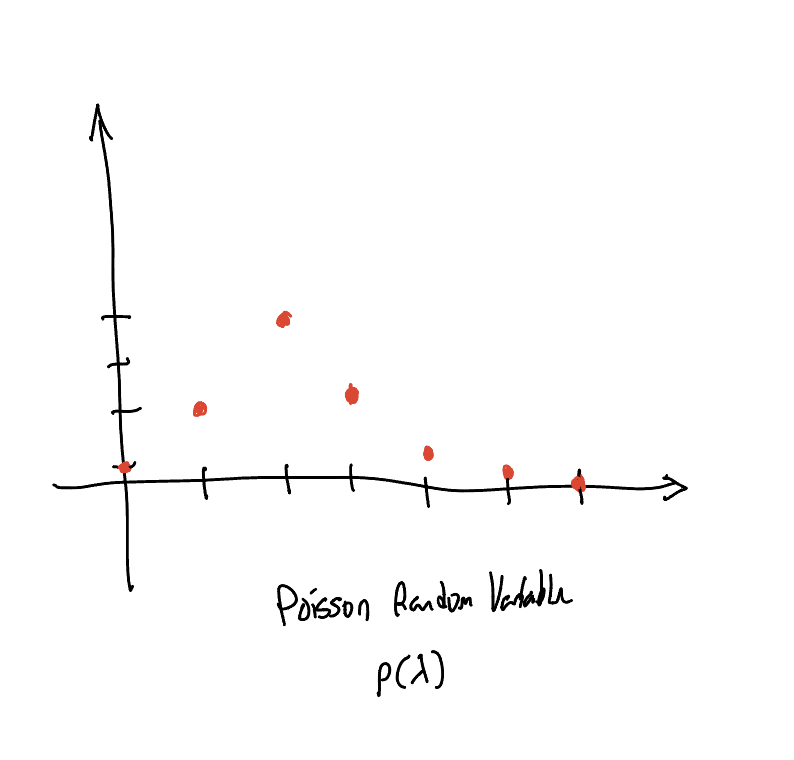
\includegraphics[height=2in]{q2.jpeg}
        \caption{pmf plot for $X \sim \rho(\lambda)$}
    \end{center}
\end{figure} 

\subsubsection{Special Properties}

There are several special properties associated with the Poisson random variable:

\begin{enumerate}
    \item Given two independent Poisson random variables $X, Y$, the sum of $M_{X+Y} = M_{\alpha+\beta}$, where $\alpha, \beta \sim \rho(\lambda)$.
    \item Poisson random variables have time homogeneity, meaning the interval on which $I$ resides can be scaled by a constant $c$ to create another Poisson random variable $Y$. For example, given a Poisson random variable $X$, we can double the time interval to create $Y$ such that $Y \sim \rho(2\lambda)$.
\end{enumerate}

\subsubsection{Typical Examples}

\begin{enumerate}
    \item The number of cars that pass a certain point in a given hour.
    \item The number of customers that arrive at a bank in a given hour.
    \item The number of defective parts that are produced in a given hour.
    \item The number of radioactive particles that decay in a given hour.
\end{enumerate}

\end{document}